\documentclass[10pt]{article}
\usepackage[utf8]{inputenc}
\usepackage[activeacute,spanish,es-nodecimaldot]{babel}
\usepackage[left=1.5cm,top=1.5cm,right=1.5cm, bottom=1.5cm,letterpaper, includeheadfoot]{geometry}
\usepackage[parfill]{parskip}

\usepackage{amssymb, amsmath, amsthm}
\usepackage{graphicx}
\usepackage{lmodern,url}
\usepackage{paralist} %util para listas compactas

\usepackage{fancyhdr}
\pagestyle{fancy}
\fancypagestyle{plain}{%
\fancyhf{}
\lhead{\footnotesize\itshape\bfseries\rightmark}
\rhead{\footnotesize\itshape\bfseries\leftmark}
}


% macros
\newcommand{\QQ}{\mathbb Q}
\newcommand{\RR}{\mathbb R}
\newcommand{\NN}{\mathbb N}
\newcommand{\ZZ}{\mathbb Z}
\newcommand{\CC}{\mathbb C}

%Teoremas, Lemas, etc.
\theoremstyle{plain}
\newtheorem{teo}{Teorema}
\newtheorem{lem}{Lema}
\newtheorem{prop}{Proposición}
\newtheorem{cor}{Corolario}

\theoremstyle{definition}
\newtheorem{defi}{Definición}
\newtheorem{eje}{Ejemplo}
\newtheorem{ejer}{Ejercicio}
% fin macros

%%%%% NOMBRE AUXILIARES Y FECHA
\newcommand{\sca}{Diego Garrido}
\newcommand{\fecha}{9 de julio  de 2020}

%%%%%%%%%%%%%%%%%%

%Macros para este documento
\newcommand{\cin}{\operatorname{cint}}


\begin{document}
%Encabezado
\fancyhead[L]{Facultad de Ciencias Físicas y Matemáticas}
\fancyhead[R]{Universidad de Chile}
\vspace*{-1.2 cm}
\begin{minipage}{0.6\textwidth}
\begin{flushleft}
\hspace*{-0.5cm}\textbf{MA4702. Programación Lineal Mixta. 2020.}\\
\hspace*{-0.5cm}\textbf{Profesor:} José Soto\\
\hspace*{-0.5cm}\textbf{Auxiliar:} \sca\\
\hspace*{-0.5cm}\textbf{Fecha:} \fecha.
\end{flushleft}
\end{minipage}
\begin{minipage}{0.36\textwidth}
\begin{flushright}

\includegraphics[scale=0.15]{fcfm}
\end{flushright}
\end{minipage}
\bigskip
%Fin encabezado

%Titulo Auxiliar
\begin{center}
\LARGE\textbf{Total Dual Integral (TDI)}
\end{center}

Sea $G=(V,E)$ un grafo conexo y no dirigido. 
El objetivo de este problema es probar que el sistema que define al polítopo de los bosques de $G$,
$B(G)=\{x\in \RR^E\colon x(E(S))\leq |S|-1, \forall\; \emptyset\neq S\subseteq V, x\geq 0\}$ es TDI.

\hspace{-15pt}\textbf{(a)} 
Escriba el dual (D) del problema $\max\{c^Tx\colon x\in B(G)\}$, usando variables $\{y_S\}_{S\subseteq V, S\neq \emptyset}$.

\textbf{Solución:}
El primal y dual son:
\begin{alignat*}{5}
(L(c))\;\max\; & c^T x & \qquad \qquad& &(D(c))\;\min \sum_{\emptyset\neq S\subseteq V}&y_S(|S|-1)\\
x(E(S))&\leq |S|-1 &\quad \forall \emptyset\neq S\subseteq V&\qquad\qquad &\sum_{S\colon \{u,v\}\subseteq S} y_S&\geq c_{uv} &\forall uv\in E\\
x_e&\geq 0 &\forall e\in E & &y_S&\geq 0& \forall \emptyset\neq S\subseteq V
\end{alignat*}


\hspace{-15pt}\textbf{(b)} Considere una solución dual óptima $y^*$ que minimice la cantidad $\Psi(y)=\sum_{S\subseteq V, S\neq \emptyset} y_S |S||V\setminus S|$
y pruebe que el soporte $\mathcal{L}$ de $y^*$ es una familia \textbf{laminar}, es decir que no existen dos conjuntos $A, B$ intersectantes en su soporte\footnote{$A, B$ se dicen intersectantes si $A\setminus B$, $B\setminus A$, $A\cap B$ son todos no vacíos.}. ¡Cuidado! Recuerde que no existe la variable $y_\emptyset$.\\

\textbf{Solución:}
Sea $\mathcal{L}$ el soporte de $y^*\in \RR^{2^V}$ y supongamos por contradicción que $A, B\in \mathcal{L}$ son intersectantes. Como $A$ y $B$ son intersectantes, $A\cap B\neq \emptyset$ así que no hay problema con hablar de la variable $y^*_{A\cap B}$.

Sea $0<\varepsilon\leq \min\{y^{*}_{A},y^{*}_{B}\}$ y definamos $\hat{y}$ como el vector obtenido de $y^*$ bajando en $\varepsilon$ el valor de $y^*_A, y^*_B$ y subiendo en $\varepsilon$ el valor de $y^*_{A\cap B}$, $y^*_{A\cup B}$.

\textbf{Paso 1:} Veamos que $\hat{y}$ es dual factible:

Por definición de $\hat{y}$ tenemos que $\hat{y}_S\geq 0$.
En lo que sigue usamos la notación de indicatriz $\IV{p}=1$ si y solo si $p$ es verdadero.
Para $uv\in E$ notamos que 
\begin{align}
\Delta:=\sum_{S\colon \{u,v\}\subseteq S} (\hat{y}_S  - y^*_S) = \varepsilon ( \IV{\{u, v\} \subseteq A\cup B} + \IV{\{u,v\} \subseteq  A\cap B}- \IV{\{u,v\}\subseteq A} - \IV{\{u,v\}\subseteq B})
\end{align}

Veamos que el lado derecho de (1) es al menos 0. Lo más sencillo es analizar los términos negativos: 

Si se tienen ambos $\{u,v\}\subseteq A$ y $\{u,v\}\subseteq B$, entonces también se tienen 
$\{u,v\}\subseteq A\cap B$ y $\{u,v\}\subseteq A\cup B$ por lo que el lado derecho es 0.

Si solo uno de $\{u,v\}\subseteq A$ y $\{u,v\}\subseteq B$ es cierto, entonces también tenemos $\{u,v\}\subseteq A\cup B$ y luego el lado derecho es 2-1 o 1-1, en cualquier caso es mayor o igual que 0.

Si ninguno de $\{u,v\}\subseteq A$ y $\{u,v\}\subseteq B$ es cierto, los términos del lado derecho son mayores o iguales que 0.

Usando (1) se concluye que $\sum_{S:\{u,v\}\subseteq S}\hat{y}_S=\Delta + \sum_{S:\{u,v\}\subseteq S}y^*_S\geq c_{uv}$. Como esto es para todo $uv\in E$ tenemos que $\hat{y}$ es dual factible.


\textbf{Paso 2:} Veamos que $\hat{y}$ es dual óptimo. Esto se tiene pues la diferencia en objetivo es
\begin{align*}
\sum_{\emptyset\neq S\subseteq V}(\hat{y}_S(|S|-1) - y^*(|S|-1)) &= \varepsilon[(|A\cup B| -1)+(|A\cap B|-1) - (|A|-1)-(|B|-1))]=0.
\end{align*}
(la igualdad a 0 se tiene por propiedad de cardinales: $|A\cup B|=|A|+|B|-|A\cap B|$)

\textbf{Paso 3:} Veamos que $\hat{y}$ tiene menor potencial que $y^*$. Esto se tiene pues
(esto se vio en clase, no es necesario probar nuevamente la segunda igualdad)
\begin{align*}
\Psi(\hat{y})-\Psi(y^*) &= \varepsilon[ |A\cup B||V\setminus (A\cup B)| + |A\cap B||V\setminus (A\cap B)| -|A||V\setminus A| -|B||V\setminus B |]\\
&= -2 \varepsilon |A\setminus B||B\setminus A|
\end{align*}
y esto es menor que 0 pues $A\setminus B, B\setminus A$ son no vacíos.


\hspace{-15pt}\textbf{(c)} Sea $W$ un conjunto finito, $\mathcal{L}\subseteq 2^W$ una familia laminar y $\mathcal{E}\subseteq 2^W$ una familia de conjuntos. Pruebe que la matriz $M\in \{0,1\}^{\mathcal{E}\times \mathcal{L}}$ dada por
$M_{I,J}=\begin{cases} 1 & \text{ si } I \subseteq J,\\ 0 &\text{ en otro caso,}\end{cases}$ es totalmente unimodular (TU)

\textbf{Indicación:} Use Ghouila-Houri asignando signos en las columnas adecuadamente.

\textbf{Solución:}

Sea $\mathcal{L}'\subseteq \mathcal{L}$ un subconjunto de columnas de la matriz $M$ y notamos que $\mathcal{L}'$ sigue siendo laminar. Asignemos valor 1 a todos los conjuntos $X$ que están incluidos en un número par de conjuntos de $\mathcal{L}'$ y -1 a todos los conjuntos incluidos en un número impar. En un dibujo, esto se ve asi:\\

\begin{figure}[h]
	\centering
	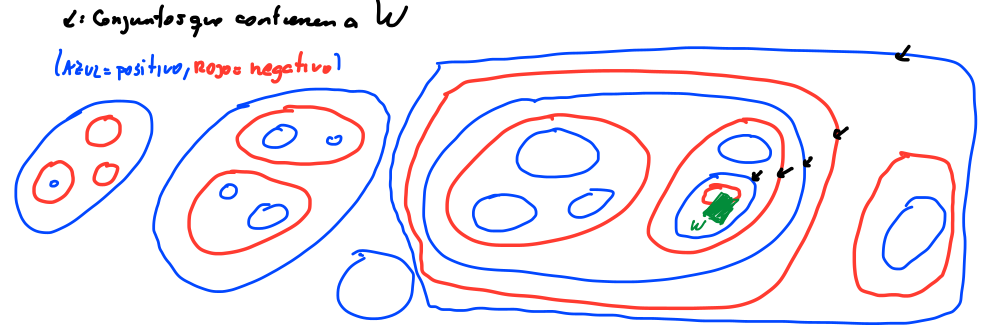
\includegraphics[width=0.8\textwidth]{laminar_set.png}
\end{figure}

Para cualquier $I$ fijo, los conjuntos de $\mathcal{L}'$ que contienen a $I$ forman una cadena:
$J_1\subseteq J_2\subseteq \dots \subseteq J_k$ y los signos de $J_1, J_2, \dots, J_k$ alternan por definición. Luego $\sum_{J}\text{signo(J)}M_{I,J}$ es 0, 1 o -1.
Por Ghoulia-Houri, la matriz $M$ es totalmente unimodular.

\hspace{-15pt}\textbf{(d)} Usando las partes (b) y (c), pruebe que el sistema que define $B(G)$ es totalmente dual integral (TDI). Concluya que $B(G)$ es integral.

\textbf{Solución:}

El sistema que define a $B(G)$ tiene datos racionales. Sea $c\in \ZZ^E$ una función objetivo con coeficientes enteros, tal que $L(c)$ es finito. De la parte (b) concluimos que el dual $D(c)$ tiene una solución $y^*$ con soporte $\mathcal{L}$ laminar. El sistema $D'(c)$ obtenido de $D(c)$ al restringirnos a las variables del soporte es de la forma $\min\{\sum_{S\in \mathcal{L}} y_S (|S|-1)\colon My\geq 0, y\in \RR^{\mathcal{L}}_+\}$ para cierta matriz $M\in \{0,1\}^{E\times \mathcal{L}}$ que cumple $M_{\{u,v\}, S}=1$ si y solo si $\{u,v\}\subseteq S$. Considerando $E$ como una familia de conjuntos (de cardinal 2) de $V$, tenemos que $M$ es de la forma considerada en la parte (c), y luego $M$ es totalmente unimodular.

Se concluye que $D'(c)$ tiene alguna solución óptima $\bar{y}$ entera. Como además el óptimo de $D(c)$ es factible en $D'(c)$ se concluye que $\bar{y}$ es óptima en $D(c)$, y luego el sistema original es TDI.

Para terminar notamos que el sistema que define a $B(G)$ tiene vector lado derecho entero. Como el sistema es TDI se concluye que $B(G)$ es polítopo integral.

\end{document}

